    The cutoff-weighted reference OU coverage is 0.8056, with
    RMSE 2.4110 and mean predictive width 5.8566. The
    observation-only Bayesian comparator has coverage 0.7222.
    For the same OU model with coefficients fixed at their marginal posterior
    medians, coverage is 0.6944; this isolates a plug-in comparison
    within that model, rather than attributing every change from the earlier
    neural fits to parameter uncertainty alone. Noise-prior sensitivity gives
    descriptive coverage ranging from 0.7778 to 0.8333.

    All reported runs meet the declared computational thresholds: the largest
    monitored $\widehat R$ is 1.0070, minimum bulk ESS is
    641, and minimum tail ESS is 444.
    These checks support finite-run numerical reliability, not model adequacy.
    The noise split and correlation time remain uncertain. The intervals in
    Table~\ref{tab:bayesian-parameters} are parameter credible intervals;
    the forecast bands in Figure~\ref{fig:bayesian-forecast} are observation
    predictive intervals. The original residual AIC/BIC scores are not used
    as Bayesian model evidence.

    All seven uncovered responses across the reference OU holdouts exceed
    their upper bounds. Mean observed-minus-predicted residuals increase from
    approximately 1.28 to 2.25 response units across the cutoffs. This pattern
    motivates investigation of structural underprediction, rather than a
    claim that parameter integration has resolved calibration. A predictive
    mixture integration check using 6000, 12000, and 24000 posterior draws at
    cutoff 132 leaves coverage unchanged; interval endpoints shift by at most
    approximately 0.012 response units relative to the 6000-draw calculation.

    The holdouts still reuse 15 distinct scalar observations across 36 forecast
    entries. A near-nominal aggregate rate would not establish calibration on
    independent future experiments. The Bayesian extension is retained as an
    exploratory observation-model comparison, and REV-07 remains open until
    predictive adequacy is established with stronger validation.

\begin{figure}[htbp]
    \centering
    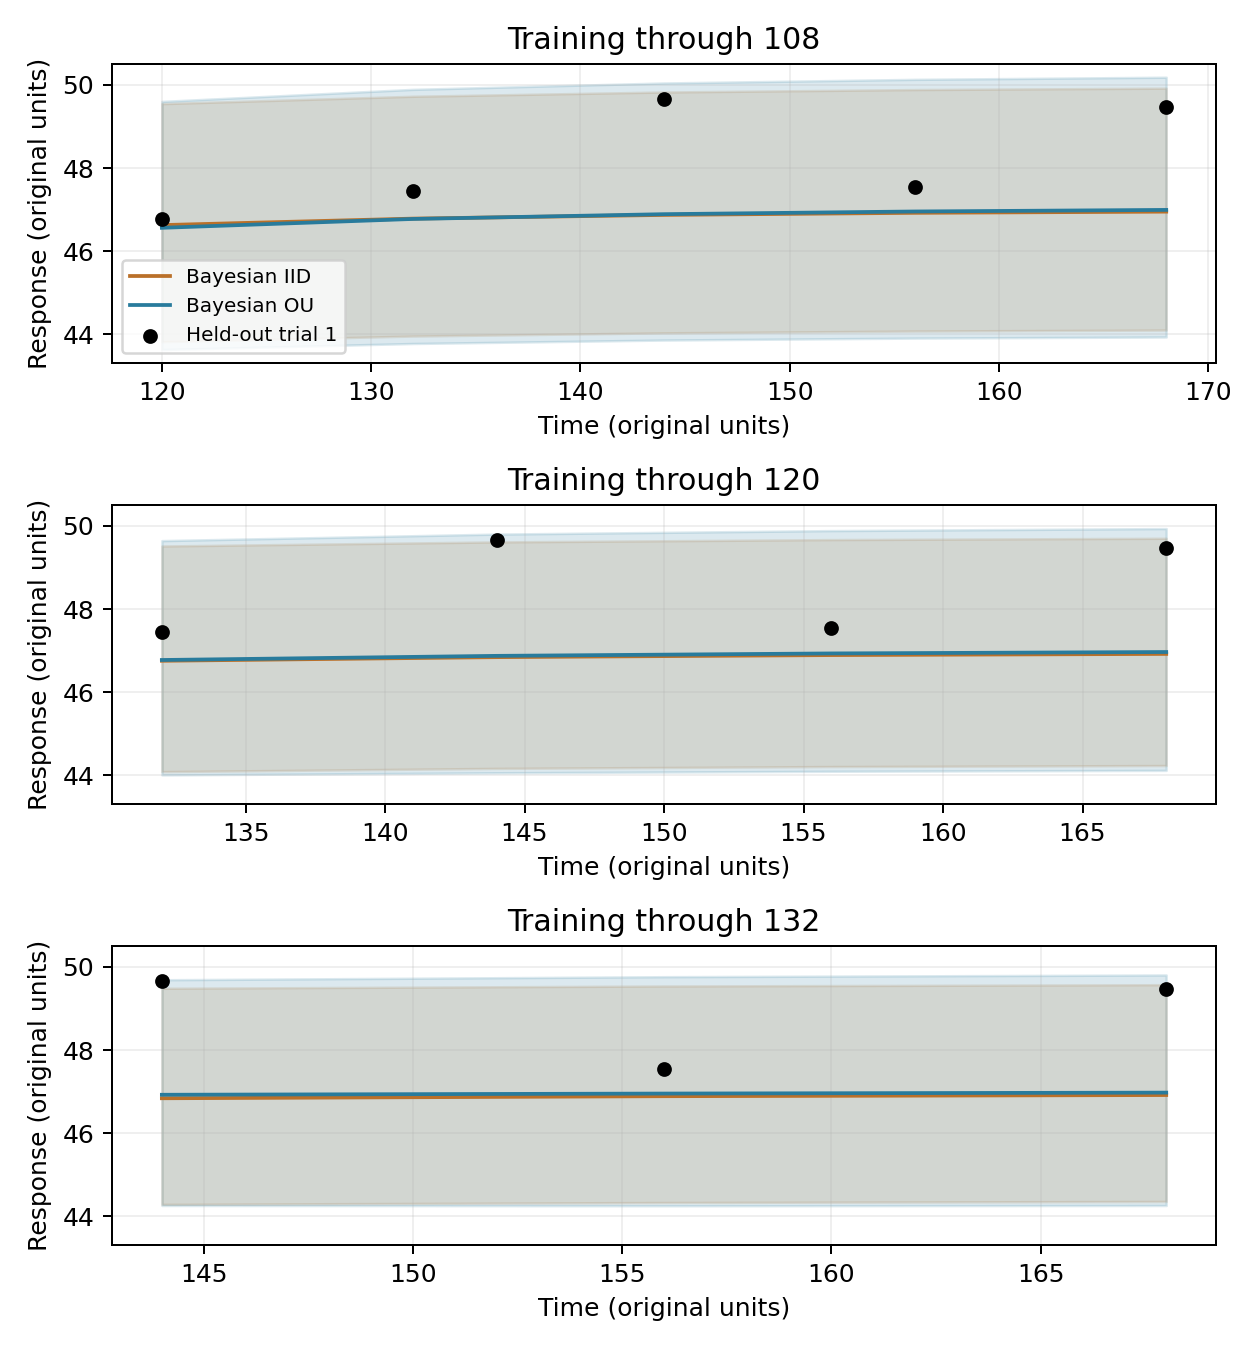
\includegraphics[width=\textwidth]{../results/bayesian/forecast_comparison.png}
    \caption{Posterior predictive means and central 90 percent observation
    intervals for trial 1. Black markers are held-out responses. Metrics use
    all three trials; intervals integrate the parameter posterior.}
    \label{fig:bayesian-forecast}
\end{figure}
\begin{figure}[htbp]
    \centering
    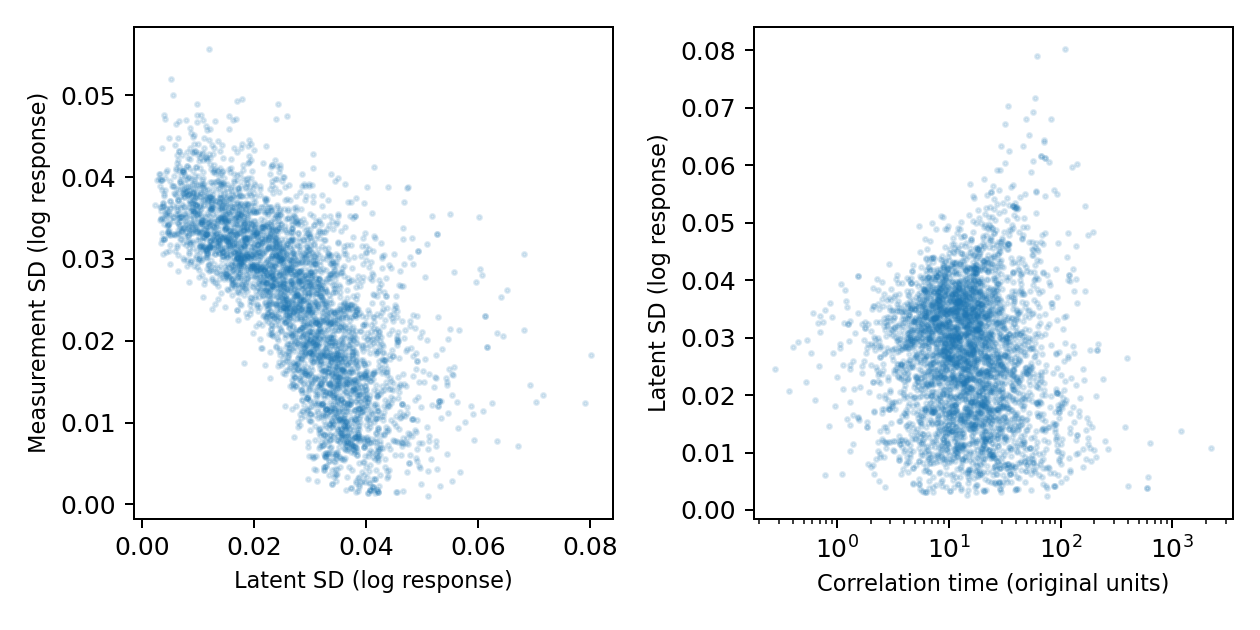
\includegraphics[width=0.9\textwidth]{../results/bayesian/noise_identifiability.png}
    \caption{Joint posterior noise and correlation parameters for the full-data
    OU model. Correlation of noise components and a broad correlation-time
    range limit a mechanistic interpretation of their separate estimates.}
    \label{fig:bayesian-identifiability}
\end{figure}
